\documentclass{article}
\usepackage{etoolbox}
\usepackage{graphicx}

\ifdef{\myoutput}{}{\def\myoutput{concept}}
\ifdef{\myversion}{}{\def\myversion{1}}

\usepackage[output=\myoutput
,numberofversions=4
,version=\myversion
,seed=4
,randomizequestions=true
,randomizeanswers=true
,writeRfile=true
]{mcexam}

\usepackage[margin=0.95in]{geometry}
\usepackage{multicol}

\usepackage{fancyhdr,lastpage}
\pagestyle{fancy}
\fancyhf{}
\renewcommand{\headrulewidth}{1pt} 
\renewcommand{\footrulewidth}{1pt}
\lfoot{\mctheversion}
\rfoot{Page \thepage\ of \pageref{LastPage}}
\lhead{Quiz 7.1 and 7.3 \mctheversion \\ MAT 2000: Introduction to Statistics}
\rhead{Name Print): \hspace{2.5 in}}

\usepackage{calc}
\renewenvironment{setmcquestion}
{\begin{minipage}[t]{\linewidth-\labelwidth}}
	{\end{minipage}\par}
	
\renewenvironment{setmcquestioninstruction}
{\begin{minipage}{\textwidth}}
	{\end{minipage}}
	
\renewenvironment{setmcanswers}{}{}
\setlist[setmcquestions]{label=\mcquestionlabelfmt{*}.
	,ref=\mcquestionlabelfmt{*}
	,itemsep=0.5\baselineskip
	,topsep=1\baselineskip
}

\renewcommand\mcversionlabelfmt[1]{\arabic{#1}}

%copy-pasting from MS Word, use regex to find [\*]*[a-d]\. and replace with \answer 

\raggedbottom

\begin{document}
	Circle the correct answer for each question.  If you're unsure, you can write numbers 1, 2, 3, etc. next to the choices to get partial credit.  Questions refer to the nonindented paragraph above unless otherwise stated.\\[.5cm]
	
	\begin{mcquestions}
		\begin{mcquestioninstruction}
			Monthly snowfall (in inches) was measured over several winters in Fort Collins, Colorado. Researchers also recorded whether the measurement was taken in the Early winter (September to December) or Late winter (January to June). Boxplots displaying the distribution of monthly snowfall for each season are below.
			\begin{center}
				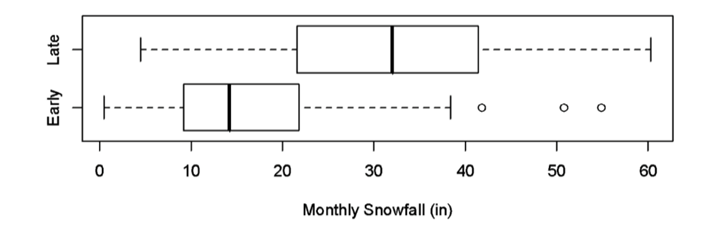
\includegraphics[width=\textwidth]{snowfall.png}
			\end{center}
			Use this to answer the next five questions:
		\end{mcquestioninstruction}
		
		\question The shape of the distribution of monthly snowfall measurements for the Early season is
		\begin{mcanswerslist}
			\answer symmetric.
			\answer[correct] skewed right.
			\answer skewed left.
			\answer bimodal.
		\end{mcanswerslist}
		
		\question[follow] What is the upper quartile (Q3) of the distribution of monthly snowfall measurements for the Late season (approximately)?
		\begin{mcanswerslist}
			\answer 22
			\answer 33
			\answer[correct] 41
			\answer 60
		\end{mcanswerslist}
		
		\question[follow] Which of the following sentences correctly interprets the first quartile (Q1) of the distribution of monthly snowfall measurements for the Early season?
		\begin{mcanswerslist}
			\answer[correct] About 25\% of Early season winter months in Fort Collins get less than 9 inches of snow.
			\answer About 50\% of Early season winter months in Fort Collins get less than 9 inches of snow.
			\answer About 75\% of Early season winter months in Fort Collins get less than 9 inches of snow.
			\answer About 25\% of Early season winter months in Fort Collins get more than 38 inches of snow.
		\end{mcanswerslist}
		
		\question[follow] Which season has the larger median monthly snowfall?
		\begin{mcanswerslist}
			\answer Early
			\answer[correct] Late
			\answer The two medians are approximately equal.
			\answer The plot does not provide enough information to determine which median is larger.
		\end{mcanswerslist}
		
		\question[follow] The boxplots demonstrate that there is an association between which two variables?
		\begin{mcanswerslist}
			\answer Early and Late winter season
			\answer Snowfall and months
			\answer[correct] Monthly snowfall and whether the time was Early or Late winter season
			\answer Whether it was Early or Late winter season and months
		\end{mcanswerslist}
		
		\question Which of the following data sets has the largest standard deviation?
		\begin{mcanswerslist}
			\answer 1, 2, 3, 4, 5
			\answer 1, 3, 3, 3, 5
			\answer[correct] 1, 1, 3, 5, 5
			\answer 1, 1, 1, 1, 1
		\end{mcanswerslist}
		
		\begin{mcquestioninstruction}
			A random sample of Hope College students was taken and one of the questions asked was how many hours per week they study.  The goal is to see whether a difference exists between males and females in terms of average study time.  The sample results are given in the following table.
			\begin{center}
				\begin{tabular}{| l | l | l |}
					\hline
					& \textbf{Female} & \textbf{Male} \\
					\hline
					\textbf{Sample Size} & 125 & 75 \\
					\hline
					\textbf{Sample Average} & 18.52 & 15.17 \\
					\hline
					\textbf{Sample SD} & 10.85 & 11.32 \\
					\hline
				\end{tabular}
			\end{center}
		\end{mcquestioninstruction}
		
		\question Assuming the distribution of study times is not strongly skewed for either sample, which approach would be more appropriate for these data: simulation-based or theory-based?
		\begin{mcanswerslist}
			\answer Simulation-based, since this approach works for any sample size.
			\answer Theory-based, since both 125 and 75 are greater than 20.
			\answer[correct] Either approach would be appropriate.
			\answer Neither approach would be appropriate.
		\end{mcanswerslist}
		
		\begin{mcquestioninstruction}
			An article that appeared in the British Medical Journal (2010) presented the results of a randomized experiment conducted by researcher Jeremy Groves, whose objective was to determine whether the weight of his bicycle could affect his travel time to work. On each of 56 days (from mid-January to mid-July 2010), Groves tossed a £1 coin to decide whether to bike to work on a carbon frame (lighter) bicycle that weighed 20.9 lbs or a steel frame (heavier) bicycle that weighed 29.75 lbs, and recorded the commute time (in minutes) for each trip.
			
			Here are the summary statistics for his data:
			
			\begin{center}
				\begin{tabular}{| l | l | l | l |}
					\hline
					\textbf{Bike Type} & \textbf{Sample size} & \textbf{Sample average} & \textbf{Sample SD} \\
					\hline
					\textbf{Carbon frame (lighter)} & 26 & 108.34 min & 6.25 min \\
					\hline
					\textbf{Steel frame (heavier)} & 30 & 107.81 min & 3.89 min \\
					\hline
				\end{tabular}
			\end{center}
		\end{mcquestioninstruction}
		
		\question Calculate the standardized statistic for the appropriate test of two means (carbon – steel).
		\begin{mcanswerslist}
			\answer 0.71
			\answer 0.53
			\answer[correct] 0.37
			\answer 1.42
		\end{mcanswerslist}
		
		\question[follow] Under the null hypothesis, what distribution does the test statistic follow?
		\begin{mcanswerslist}
			\answer Standard normal distribution
			\answer[correct] t-distribution
			\answer Skewed distribution
			\answer Normal distribution
		\end{mcanswerslist}
		
		\begin{mcquestioninstruction}
			In order to investigate whether talking on cell phones is more distracting than listening to car radios while driving, sixty-four student volunteers (from a single college class) were randomly assigned to a cell phone group or a radio group (32 students were assigned to each group). Each student ``drove'' a machine that simulated driving situations. While ``driving'' the simulator, a target would flash red at irregular intervals. Participants were instructed to press the ``brake'' button as soon as possible when they detected a red light. Participant response times were measured as the time between the red light appearing and pushing the brake button. While driving, the radio group listened to a radio broadcast and the cell phone group carried on a conversation on the cell phone with someone in the next room.
		\end{mcquestioninstruction}
		
		\question The theory based 99\% confidence interval for $\mu_{{cell}}-\mu_{{radio}}$ is given by $(-0.7401,103.7401)$. Does the interval provide significant statistical evidence that the long-run mean response time differs between the cell phone and radio treatments?
		\begin{mcanswerslist}
			\answer Yes, since most of the interval is positive.
			\answer Yes, since zero is not contained in the interval.
			\answer[correct] No, since zero is contained in the interval.
			\answer The interval does not provide enough information to answer this question.
		\end{mcanswerslist}
		
		
	\end{mcquestions}
\end{document}